%%%%%%%%%%%%%%%%%%%%%%%%%%%%%%%%%%%%%%%%%%%%%%%%%%%%%%%%%%%%
%%%  Augmenting TV Newscasts via Entity Expansion  %%%
%%%%%%%%%%%%%%%%%%%%%%%%%%%%%%%%%%%%%%%%%%%%%%%%%%%%%%%%%%%%

\documentclass{llncs}

\newcommand{\superscript}[1]{\ensuremath{^{\textrm{#1}}}}

\usepackage{makeidx}  % allows for indexgeneration
\usepackage[hyphens]{url}
\usepackage{textcomp}
\usepackage{color}
\usepackage{listings}
\usepackage{multirow}
\usepackage{mathtools}
\usepackage{graphicx}
\usepackage{fancyvrb}
\usepackage{amsmath}
\usepackage{graphicx}
\usepackage[font=small,labelfont=bf]{caption}
\setcounter{MaxMatrixCols}{20}
\usepackage{pbox}
\usepackage{amsfonts}

\setlength{\belowcaptionskip}{-30pt}

% listing styles
\lstset{numbers=left, numberstyle=\tiny,basicstyle=\ttfamily\scriptsize, tabsize=2, keywordstyle=\underbar, stringstyle=\small, backgroundcolor=\color[gray]{0.94}, framexleftmargin=2pt}
\lstdefinestyle{rdfa}{numberblanklines=true, morekeywords={}}


\begin{document}
\frontmatter          % for the preliminaries
\pagestyle{headings}  % switches on printing of running heads
\mainmatter              % start of the contributions

\title{Detecting and Displaying Hot Spots in Web Videos}
\author{Jos\'e Luis Redondo Garc\'ia\inst{1}, Mariella Sabatino\inst{1}, Pasquale Lisena\inst{1}, Rapha\"el Troncy\inst{1}}
\institute{
EURECOM, Sophia Antipolis, France, \\
\email{\{redondo, mariella.sabatino, pasquale.lisena, raphael.troncy\}@eurecom.fr}
}

\maketitle              % typeset the title of the contribution

%%%%%%%%%%%%%%%%%%
%%%  Abstract  %%%
%%%%%%%%%%%%%%%%%%

\begin{abstract}
This paper presents an approach for identifying relevant fragments (called Hot Spots) inside educational online videos that combines visual analysis techniques and the knowledge from the Web in order to get a quick overview about the content and promote a media consumption at a higher level of granularity. 

We perform a first segmentation by combining visual features and semantic units in transcripts (paragraphs). The resultant fragments are semantically annotated via Named Entity Extraction and Topic detection. After identifying consecutive chapters talking about similar topics and entities, we merge them into bigger and semantic independent media units. Finally we rank them, filter out the lower scored candidates, and propose a summary that illustrates the Hot Spots on the dedicate media player. An online demo is available at \url{http://linkedtv.eurecom.fr/mediafragmentplayer}.

\keywords{Semantic Video Annotation, Media Fragments, Summarization}
\end{abstract}

%%%%%%%%%%%%%%%%%%%%%%%%%
%%%  1. Introduction  %%%
%%%%%%%%%%%%%%%%%%%%%%%%%

\section{Introduction}

Today people consume all kind of audiovisual content on a daily basic. From breaking news to satiric videos passing by a tutorial on how to cook that wonderful meal, we are constantly bombarded with all kind of multimedia documents. In this media-overloaded scenario it becomes hardly complicated for us to decide if a candidate video is really worth to be watch, or which are the fragments that can be potentially relevant for us without having to watch the entire video.

This phenomena is equally evident when it comes to curated, editorial and educational Web videos. Some studies made over media entertainment streaming services~\cite{Yu2006} reveal that the majority of partial content views (52.55\%) are terminated by the user within the first 10 minutes, and about a 37\% of these sessions do not last past the first five minutes. In practice, it is difficult and time consuming to manually gather video insights that give the viewers a fair understanding about what the video is talking about. Our research tackles this inconvenience by proposing a set of automatically annotated media fragments called Hot Spots, which intend to highlight the main ideas of the video and make easier for the user to decide which fragment can be relevant for him to watch or share.

%Segmentation of videos
The challenge of video segmentation has been addressed by many previous research approaches. Some of them rely exclusively in visual and low-level features like color histograms or visual concept detection clustering operations~\cite{snoek2005multimodal}. On the other hand, there are some pure text�based implementations which leverage in the transcripts and written annotations that goes together with the video, like for example~\cite{chang1992image}. 
%A special variety of the latter tries to go further and study the semantic behind the text by identifying relevant concepts and linking them to a taxonomy, like in~\cite{de2013ghent}. 
Finally, there are some initiatives that combine different kinds of techniques~\cite{chang2005combining} in order to exploit the best of each. Our demo fits into this last category, with the added value of leveraging on the Web: it is applicable over online videos and it relies on structured knowledge when analyzing and annotating them. 

% Semantic
%Concerning the multimedia annotation, one of the main approaches consists on running Named Entity Recognition (NER) over the textual information attached to particular video fragment. Those techniques are an essential component within the Information Extraction field that focus on: identifying atomic information units in texts, named entities; classifying entities into predefined categories (also called context types) and linking to real world objects using web identifiers (Named Entity Disambiguation). A growing number of APIs provide such a service, like AlchemyAPI\footnote{\fontsize{8pt}{1em}\selectfont \url{http://www.alchemyapi.com/}} or DBpedia Spotlight\footnote{\fontsize{8pt}{1em}\selectfont \url{http://spotlight.dbpedia.org/}}.

%%%%%%%%%%%%%%%%%%%%%%%%%%%%%%%%%%
%%%  Generating and Displaying Hot Spots in Web Videos    %%%
%%%%%%%%%%%%%%%%%%%%%%%%%%%%%%%%%%

\section{Generating and Displaying Hot Spots in Web Videos}
\label{sec:hotspots}

This demo implements a multimodal algorithm for detecting key fragments in a set of 1681 TED talks and annotating them in order to have a quick overview about which are the main topics involved.

%%%  Media Fragments Generation %%%
\subsection{Video Segmentation}
\label{sec:fragmentsgeneration}

In first place we perform a video segmentation based only in pure visual features. The resultant fragments, called Shots, are considered like the smaller visually-consistent video chunks. The algorithm used in our approach has been described in~\cite{sidiropoulos2011temporal}. However semantically speaking those shots are too small: a visual change in the frame flow does not necessary reveal a disruption in what is being told on the video. We therefore introduce the notion of Chapters for naming wider chunks illustrating particular topics inside the entire video context. In order to obtain such fragments we have leveraged in some marks embedded in the available video transcripts that indicate the start of a new paragraph. As paragraphs are indeed self-contained units of a discourse dealing with a particular point or idea \footnote{\fontsize{8pt}{1em}\selectfont \url{http://en.wikipedia.org/wiki/Paragraph}}, those fragment become semantically valid for us at this point. 

In a last step those fragments are combined with visual Shots for getting the best of both techniques. In particular we extend Chapters back and forward in time in order to include complete Shots and produce semantically independent segments with visually consistent borders.

%%%  Annotating Web Videos %%%
\subsection{Media Fragment Annotation}
\label{sec:videoannotation}

Once the video has been segmented the resultant fragments are analyzed and annotated. We will rely on the textual information (subtitles) available for the 1681 TED talks in order to detect two kind of semantic clues: topics (prominent matters the video is talking about) and Named Entities taking part in the story. For the former we have used TextRazor\footnote{\fontsize{8pt}{1em}\selectfont \url{https://www.textrazor.com/documentation}}, while for the latter we used the NERD framework~\cite{Rizzo2012b}. 

Both entities and topics come accompanied by a relevance score which indicates the importance of that particular semantic unit inside the whole context of the video story. Every item detected is then mapped to the Chapter that comprises the subtitle block where the word has been mentioned. The output of this phase is a list of Chapters individually annotated with named entities (according to the NERD Ontology\footnote{\fontsize{8pt}{1em}\selectfont \url{http://nerd.eurecom.fr/ontology/nerd-v0.5.n3}}) and topics. 

% TODO Figure of a timeline with chapters and annotations being shown (probably not enough space)

\subsection{Hot Spots Generation}
\label{sec:hotspots}

At this point chapters have their own demarcated semantic information. But sometimes the semantic descriptions between temporally close chunks are similar enough to be considered as a single unit, either because they talk about the same topics or because they mention the same named entities. In order to tackle this phenomena we apply a clustering algorithm over the chapters, which accumulatively merges of consecutive similar fragments.
In order to perform this operation we apply a similarity function between consecutive pairs of chapters until no new merges are possible. This comparison leverages on the annotations attached to each segment by analyzing the number of coincidences between the topics $T = max_{3}\left \{ \sum_{topic_{i}} Rel_{i} \right  \}$ and entities $E = max_{5W's}\left \{ \sum_{entity_{i}} Rel_{i} \right  \}$: 

\begin{equation}
\begin{split}
d\left ( Ch_{1} , Ch_{2} \right ) = w_{topic}\cdot \left ( \frac{\left | T_{1} \bigcap T_{2} \right |}{max \left \{ \left | T_{1} \right |, \left | T_{2} \right |\right \}} \right ) + w_{entity}\cdot \left ( \frac{\left | E_{1} \bigcap E_{2} \right |}{max \left \{ \left | E_{1} \right |, \left | E_{2} \right |\right \}} \right ) \\
\end{split}
\end{equation}
 
After clustering process is finished the chapters have grown in length and decreased in number, but there are still too many candidates which should not be proposed as Hot Spots. Therefore we filter those fragments which contain potentially less decisive topic and entities. We define the a function for measuring the relevance of a video segment, which directly depends on the relevance and frequency of the main annotations and is inversely proportional to its length. In our current approach, the Hot Spots are those fragments whose relative relevance falls under the first quarter of the final score distribution.

%\begin{equation}
%\begin{split}
%Relevance\left ( Ch \right ) = \frac {w_{topic}\cdot \sum_{t \in T} Rel_{t} + w_{entity}\cdot \sum_{e \in E} Rel_{e}}{Duration(Ch)} \\
%\end{split}
%\%end{equation}
  
In a last step, for each Hot Spot we also generate a summarization to be shown in the dedicated media player. Again, we take advantage of the previously calculated main topics $T$ and main entities $E$.
  
%%%  Use Case: TED talks %%%
\subsection{Displaying Hot Spots for TED Talks}
\label{sec:usecase}

The obtained Hot Spots and their summaries are visualized in a user friendly MediaFragment URI \footnote{\fontsize{8pt}{1em}\selectfont \url{http://www.w3.org/TR/media-frags/}} compliant media player. The procedure to get Hot Spots available for a certain Ted talk goes like follows: after introducing a valid URL, we land in the video page from where the hot spot detection can be launch for the first time (see Figure~\ref{fig:demoScreenShots}a). When results are available, the corresponding fragments get highlighted on the timeline together with the label of the most relevant chapter annotation. This brief description can be extended to the broader set of main entities and topics in order to get a more exhaustive summary (see Figure~\ref{fig:demoScreenShots}c). Finally as shown in Figure~\ref{fig:demoScreenShots}d you can always relive that part of the talk you like the most or you would like to share with others. 

\begin{figure}[h!]
\centering
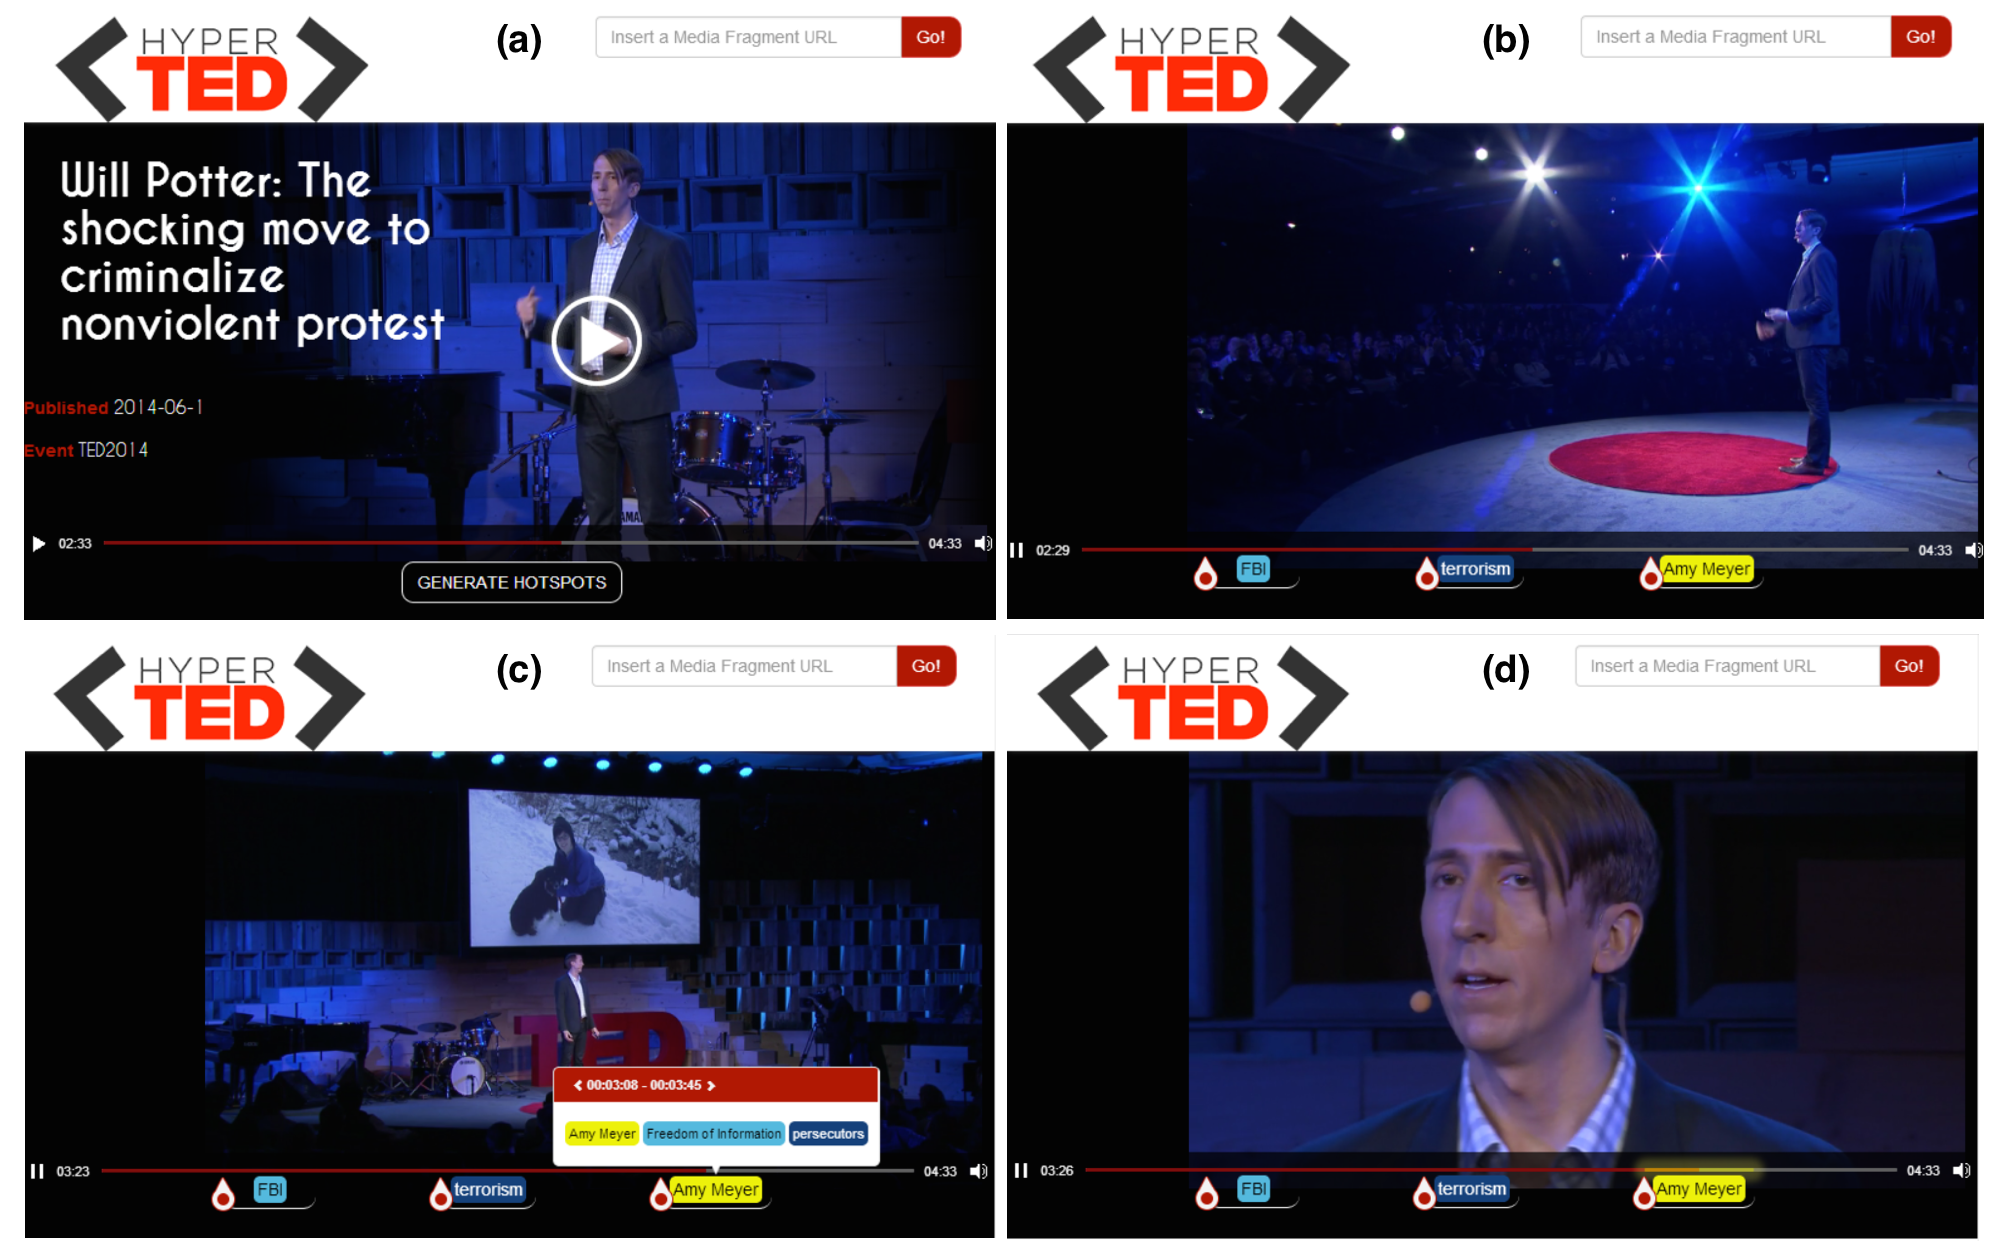
\includegraphics[width=1\textwidth]{figure/Ted_U}
\caption{Visualizing the Hot Spots of a TED Talk (available at \fontsize{8pt}{1em}\selectfont \protect\url{http://linkedtv.eurecom.fr/mediafragmentplayer/video/bbd70fff-e828-4db5-80d0-1a4c9aea430e})}
\label{fig:demoScreenShots}%\end{figure}
\end{figure}

%%%%%%%%%%%%%%%%%%%%%%%
%%%  4. Discussion  %%%
%%%%%%%%%%%%%%%%%%%%%%%

\section{Discussion}
\label{sec:discussion}

We have presented a demo tool for automatically discovering Hot Spots in online and educational videos. We leverage in a visual analysis of the multimedia content and in the knowledge available on Web for detecting which fragments illustrate the main topics in the video. Those Hot Spots allow the viewer to quickly decide if the video is interesting for him and will incentive a more fine-grained consumption in the form of media fragments. In addition, Hot Spots are visualized in a Web media player which also display the corresponding semantic annotations. 

Regarding upcoming research efforts in this same line  we plan to carry out an exhaustive evaluation of our solution involving real users feedback, in order to optimize the results of our Hot Spot generation algorithm and to improve the usability and efficiency of the developed interface. In addition in future developments we plan to further exploit the segmentation results and their corresponding annotations for establishing links between fragments belonging to different videos so the user can easily jump between fragments which seem to share a certain semantic similarity. 

%%%%%%%%%%%%%%%%%%%%%%%%%
%%%  Acknowledgments  %%%
%%%%%%%%%%%%%%%%%%%%%%%%%

\section*{Acknowledgments}
This work was partially supported by the European Union's 7th Framework Programme via the project LinkedTV (GA 287911).

%%%%%%%%%%%%%%%%%%%%%%
%%%  Bibliography  %%%
%%%%%%%%%%%%%%%%%%%%%%
\bibliographystyle{abbrv}
\bibliography{VideoHotSpots-reduced}

\end{document}
